\documentclass{diploma}

\student{Назарова Анастасия Игоревна}
\group{М8О-408Б-19}
\theme{Внедрение и контроль выполнения алгоритмов оказания медицинской помощи в web-приложение onmp.ru}

\supervisor{Пивоваров Дмитрий Евгеньевич}
\firstConsultant{---}
\secondConsultant{---}
\reviewer{---}

\faculty{№ 8 <<Компьютерные науки и прикладная математика>>}
\department{806}
\speciality{01.03.02 <<Прикладная математика и информатика>>}
\profile{Информатика}

\departmentFullName{№ 806}
\headOfDepartment{Крылов Сергей Сергеевич}

% Дата. Оставляем пустое место для дня
\date{\uline{\hspace{24pt}} мая \the\year\ года}

\newacronym{api}{API}{Application Programming Interface}
\newacronym{http}{HTTP}{Hypertext Transfer Protocol}
\newacronym{maui}{MAUI}{Multi-platform App UI}
\newacronym{mvvm}{MVVM}{Model-View-ViewModel}
\newacronym{rest}{REST}{Representational State Transfer}
\newglossaryentry{id1}{ % Нужны разные id, можно ставить просто последовательно
    name={Backend},
    description={логика работы сайта, скрытая от пользователя} 
}
\newglossaryentry{id2}{
    name={МКБ},
    description={Международная классификация болезней} 
}
\newglossaryentry{id3}{
    name={$S^{2}$},
    description={формула в списке обозначений} 
}


\addbibresource{main.bib}

% Иллюстрации всегда по центру
\makeatletter
\g@addto@macro\@floatboxreset\centering
\makeatother

\begin{document}
    \maketitle

    % \includepdf[pages=-]{extra/task} % Задание
    \setcounter{page}{2} % Устанавливает счётчик страниц

    \abstract % Структурный элемент: РЕФЕРАТ

 % Реферат

    \tableofcontents % Содержание 
    \termsanddefenitions % Термины и определения
    \listofabbreviations % Перечень сокращений и обозначений
 
    \introduction % Структурный элемент: ВВЕДЕНИЕ

Актуальность данной работы связана с необходимостью оптимизации процесса работы врачей из отделения неотложной медицинской помощи, особенно тех, которые выезжают на вызовы с использованием машин скорой помощи. В настоящее время эти медицинские специалисты заполняют бумажные карты вызова во время осмотра пациента на дому. Однако, такой подход требует ношения с собой больших объемов бумажной документации, что требует больших затрат времени и ресурсов на их заполнение, обработку и хранение.

Переход к электронному заполнению карт вызова имеет ряд значительных преимуществ. Прежде всего, медицинским работникам будет значительно удобнее носить с собой меньшее количество объемной макулатуры, так как электронная форма позволит им быстро и удобно заполнять карты вызова с использованием мобильных устройств, которые они всегда имеют под рукой. Это значительно повысит мобильность и гибкость работы медицинского персонала, позволяя им быстро и эффективно заполнять и обрабатывать данные.

Второе преимущество заключается в возможности хранения электронных карт вызова в интернете. Вместо физического хранения и поиска бумажных документов, медицинские работники смогут сохранять все карты вызова в электронном виде, обеспечивая быстрый и удобный доступ к ним из любого места. Это также позволит легко распечатывать необходимые карты вызова в случае необходимости, например, для передачи другим специалистам или для ведения медицинской документации.

Основной целью данной работы является разработка клиентской части web-сервиса с использованием технологии React.js. Это позволит создать современный и интуитивно понятный пользовательский интерфейс, который облегчит заполнение карт вызова, ускорит процесс ввода данных и повысит эффективность работы медицинских работников.

Был проведен анализ требований к функциональности и пользовательскому интерфейсу web-сервиса, разработана архитектура решения, реализованы необходимые компоненты и проведено тестирование системы. Также была осуществлена интеграция клиентской части с серверной частью системы для обеспечения полной функциональности и взаимодействия с данными.

В рамках данной исследовательской работы можно определить следующие задачи:
\begin{itemize}
    \item Анализ требований к клиентской части web-сервиса: Эта задача включает в себя изучение требований, предъявляемых заказчиком к функциональности и дизайну клиентской части web-сервиса. Необходимо провести тщательный анализ требований, чтобы полноценно понять ожидания и потребности заказчика.
    \item Проектирование клиентской части: Включает разработку детального плана и архитектуры клиентской части web-сервиса. Эта задача включает определение структуры компонентов, взаимодействия между ними, выбор подходящих библиотек и фреймворков для разработки, а также определение способа организации данных и обработки событий.
    \item Разработка функционала авторизации и аутентификации: Данный функционал позволит медицинским работникам входить в систему с использованием уникальных учетных данных. Каждому пользователю будет предоставлен доступ к рабочей среде, где они смогут создавать и использовать собственные шаблоны, а также просматривать и заполнять свои собственные карты вызова.
    \item Создание интерфейса для заполнения и сохранения карт вызова: Разработка пользовательского интерфейса, позволяющего медицинским работникам вводить информацию о состоянии здоровья пациента, тем самым заполняя карту вызова. Данные должны быть легко вводимы и интуитивно понятны, чтобы ускорить процесс заполнения.
    \item Реализация функционала хранения и организации карт вызова в папках: Готовые, Незавершенные, Архив, Шаблоны. Для организации и удобного отображения карт вызова. Это позволит медицинским работникам быстро найти и просмотреть необходимые карты вызова в соответствующих категориях.
    \item Разработка функционала создания и использования шаблонов: Реализация возможности создания шаблонов для быстрого использования частично заполненных карт вызова. Создавая шаблон, пользователь заполняет только некоторые поля карты, чтобы в дальнейшем использовать данный шаблон как основу для карты вызова.
    \item Реализация Функционала поиска, группировки и сортировки карт вызова: Предоставление возможности быстрого поиска нужной информации на основе различных параметров, таких как дата, название карты. Кроме того, группировка и сортировка карт вызова позволят легко ориентироваться в большом объеме данных, что значительно упростит процесс поиска нужной информации.
    \item Тестирование и отладка системы: Проведение тестирования для проверки функциональности и корректности работы системы. Исправление ошибок и устранение неполадок для обеспечения стабильной работы web-сервиса.
\end{itemize}


В данной работе разработка клиентской части web-сервиса осуществляется с использованием React.js - популярной JavaScript-библиотеки для построения пользовательских интерфейсов. React.js предоставляет эффективные инструменты и подходы для создания интерактивных веб-приложений с удобной обработкой данных и переиспользуемыми компонентами. Данная библиотека базируется на концепции компонентного подхода, где пользовательский интерфейс разбивается на независимые компоненты, каждый из которых может иметь свою логику и состояние. Компоненты могут быть переиспользованы, что упрощает разработку и обслуживание приложения.

Дополнительным инструментом к React был выбран Redux. Это библиотека JavaScript, которая предоставляет инструменты для управления состоянием приложения. Она является популярным выбором для разработки сложных и масштабируемых приложений, особенно тех, которые имеют большое количество взаимосвязанных данных.

Redux основывается на концепции однонаправленного потока данных и централизованного хранилища состояния. Вместо того чтобы хранить состояние внутри компонентов, Redux предлагает вынести состояние в отдельное хранилище. Компоненты могут получать доступ к состоянию из хранилища и обновлять его, используя специальные функции.

В целом, совместное использование React и Redux позволяет создавать масштабируемые, предсказуемые и легко поддерживаемые приложения с удобным управлением состоянием \cite{React&Redux}. 

Помимо этого, был выбрана библиотека Axios, которая предоставляет удобный интерфейс для выполнения HTTP-запросов из браузера. Она позволяет взаимодействовать с внешними API, отправлять запросы на сервер и обрабатывать полученные ответы.

Главная цель Axios - упростить и сделать более эффективной работу с HTTP-запросами. Она предоставляет простые методы для отправки различных типов запросов, таких как GET, POST, PUT, DELETE и другие. Кроме того, Axios предоставляет возможности для установки заголовков запроса, обработки ошибок, использования интерсепторов и других функций.

Разработка данного сервиса основывалась на архитектурной методологии Feature-Sliced Design, которая помогает структурировать код и организовать проект на основе функциональных возможностей. Она призвана улучшить масштабируемость, переиспользуемость и поддерживаемость кодовой базы. Основная идея данной методологии заключается в том, что проект разбивается на слои, каждый из которых имеет свою "зону ответственности". Каждый модуль содержит все необходимые компоненты, состояние, стили и логику, связанные с этой функциональностью. Это позволяет разработчикам работать над каждой фичей независимо друг от друга.

Результатом данной работы будет функциональный web-сервис, предоставляющий возможность электронного заполнения и хранения карт вызова для медицинских работников из отделения неотложной помощи. Ожидается, что данное решение значительно улучшит процесс работы медицинских учреждений, сократит временные затраты на бумажную работу и повысит качество медицинской помощи пациентам.

Таким образом, данная дипломная работа имеет практическую значимость и является важным шагом в совершенствовании сферы оказания неотложной медицинской помощи, предлагая инновационное решение, которое отсутствует на рынке.
 % Введение

    % Название разделов -- все прописные
\section{ПОСТАНОВКА ЗАДАЧИ}

\subsection{Потребность в разработке электронных справочных материалов}

Врачи скорой помощи на каждый вызов вынуждены носить с собой много аппаратуры для обеспечения правильной диагностики и лечения пациентов. Это может быть как медицинское оборудование, так и различные инструменты, которые могут понадобиться в ходе работы. 


Несмотря на то, что в современном мире развитие технологий набирает оборот и медицинская аппаратура постоянно модернизируется, она все равно занимает много места и является достаточно тяжелой. Багаж работника скорой помощи весит около 6-7 кг. Там хранятся ампулы, таблетки, кровоостанавливающий жгут, зажим, пинцет и т.д.. Помимо этого врачи с собой носят карты вызовов скорой медицинской помощи. Они оформляются при каждом выезде бригады скорой помощи. Зачастую врачи работают в экстремальных ситуациях, где каждая секунда на счету. В таких условиях достаточно трудно и неудобно носить большое количество аппаратуры.


Также врачи с собой носят справочники. Они содержат информацию о диагнозах, протоколах оказания медицинской помощи и других медицинских стандартах. В этих справочниках указана информация о МКБ-кодировании, что позволяет врачам быстро и точно определить диагноз и выбрать наиболее подходящий протокол оказания медицинской помощи. Кроме того, справочные материалы содержат информацию о порядке оказания первой медицинской помощи в различных ситуациях, включая остановку сердца, инсульт, аллергические реакции и другие чрезвычайные ситуации. Поэтому врачам зачастую тяжело носить столько тяжелых вещей на каждый вызов.


Одним из возможных решений этой проблемы стали портативные планшеты. В настоящее время справочники для врачей скорой помощи часто представлены в электронном виде и могут быть доступны на планшетах и других мобильных устройствах. Это позволяет врачам быстро находить необходимую информацию и использовать ее для принятия решений на месте вызова, что повышает эффективность оказания помощи.
Вот еще несколько преимуществ портативных планшетов в сравнении с традиционными бумажными справочниками :
\begin{itemize}
    \item электронные справочники легко обновляются и актуализируются по мере появления новых медицинских стандартов и протоколов, поэтому врачи могут быть уверены в том, что они работают с актуальной на данный момент информацией;
    \item с электронными справочниками можно создавать резервные копии данных и сохранять их в защищенном хранилище. Это защищает информацию от потери или повреждения и обеспечивает возможность восстановления данных при необходимости.
\end{itemize}
	По итогу хочется заметить, что использование электронных справочников в предоставит врачам скорой помощи широкий спектр инструментов и функций для оптимизации процесса оказания помощи и улучшения качества медицинского обслуживания.

\subsection{Обзор существующих решений}

Существует достаточное количество как мобильных приложений, так и веб-приложений для врачей, которые могут помочь им в работе.

Проведем анализ и обзор некоторых из них, также выявим их недостатки:

\begin{enumerate}
    \item Мобильное приложение <<Справочник Врача: МКБ-10, РЛС>>
    Данное приложение является достаточно полезным и нужным инструментом для врачей, который помогает в работе. Приложение включает в себя данных о лекарственных средствах, включая информацию о препаратах, их дозировках, побочных эффектах, взаимодействиях и противопоказаниях. Врачи могут использовать эту информацию для подбора правильного лекарственного средства для пациента, оценки безопасности и эффективности лекарств и предотвращения нежелательных реакций. Также там присутсвуют разделы об анализах, справочнике МКБ.Врачи могут использовать это для поиска и проверки правильности диагнозов, а также для стандартизации и согласования кодов диагнозов для медицинской документации и статистики.

    На рисунке~\ref{fig:fig03} приведен главный экран мобильного приложения <<Справочник Врача: МКБ-10, РЛС>>.
    
    \begin{figure}
        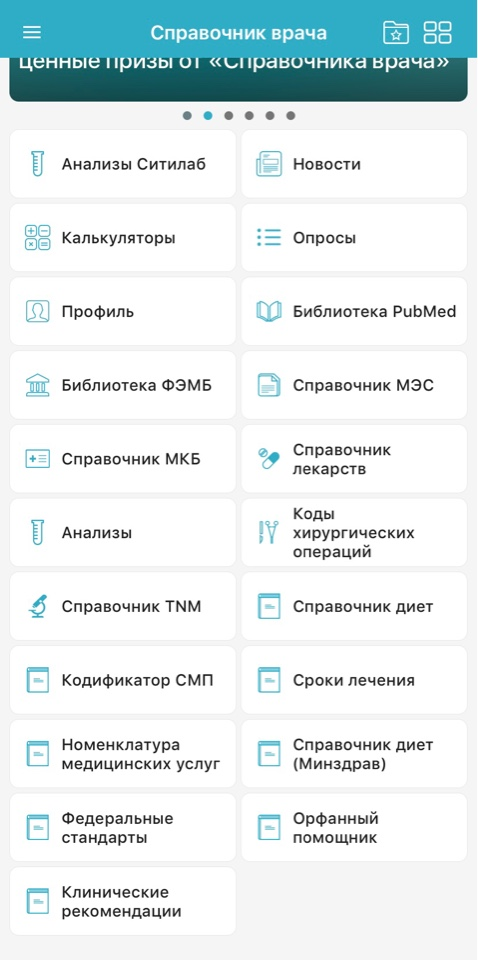
\includegraphics[scale=0.6]{styles/diploma/inc/prog1.jpeg}
        \caption{Главная страница приложения <<Справочник Врача: МКБ-10, РЛС>>}
        \label{fig:fig03}
    \end{figure}

    На рисунке~\ref{fig:fig04} приведено боковое меню мобильного приложения <<Справочник Врача: МКБ-10, РЛС>>.
     \begin{figure}
        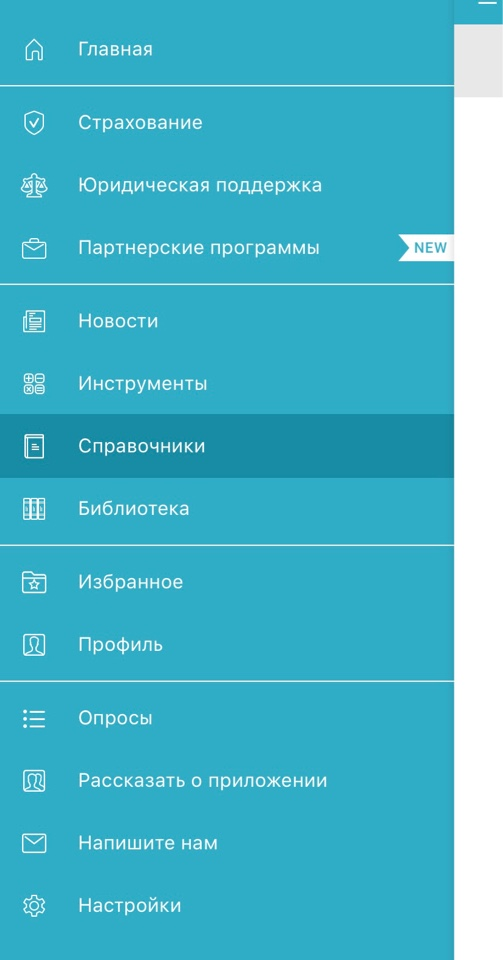
\includegraphics[scale=0.6]{styles/diploma/inc/prog2.jpeg}
        \caption{Боковое приложения <<Справочник Врача: МКБ-10, РЛС>>}
        \label{fig:fig04}
    \end{figure}
    
    Недостатки данного приложения:
    \begin{itemize}
        \item врач скорой помощи не сможет заполнять и хранить в нем карты пациентов. Т.е. это приложение предоставляет только справочную информацию;
        \item неудобный и избыточный интерфейс. Интерфейс перегружен: запутанное меню, сложная структура приложения, то есть для поиска нужной информации нужно затрачивать больше времени. Излишняя информация: (новости, опросы) на главной странице приложения.

        Плохая организация данных: если ты зашел в раздел МКБ, то для того, чтобы попасть в другой раздел, сначала необходимо перейти в боковое меню (рисунок~\ref{fig:fig04}  ), затем перейти на главную страницу, после чего выбрать нужный раздел (т.е. нет удобной навигации по разделам);
        
        \item в приложении не предусмотрена какая-либо информация об алгоритмах оказания медицинской помощи.
    \end{itemize}
    \item Бот в Telegram Paramedic
    Предоставляет довольно ограниченный функционал. Там можно получить информацию только по алгоритмам оказания скорой помощи, кодам МКБ и порядку заполнения карты вызова.
    
    На рисунке~\ref{fig:fig05} приведены справочные материалы, которые может предосталвять Telegram bot <<Paramedic>> в Москве.
    \begin{figure}
        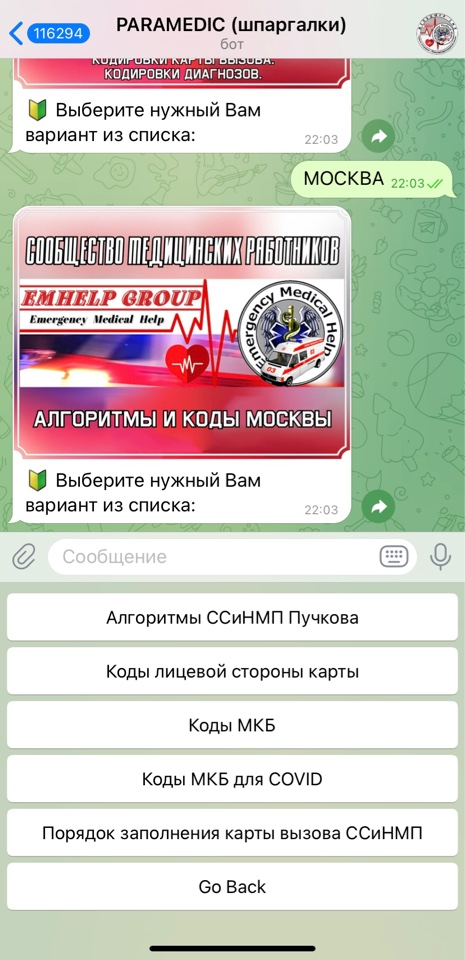
\includegraphics[scale=0.6]{styles/diploma/inc/prog2_1.jpeg}
        \caption{Telegram bot <<Paramedic>>}
        \label{fig:fig05}
    \end{figure}

    На рисунке~\ref{fig:fig06} приведены разделы медицины, которые содержит бот.Также показано, в каком виде он предоставляет информацию по алгоритмам.

     \begin{figure}
        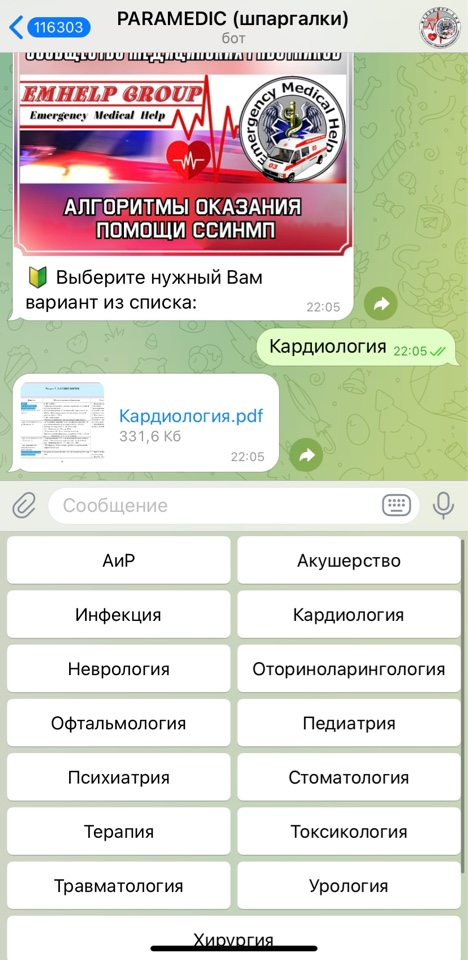
\includegraphics[scale=0.6]{styles/diploma/inc/prog2_2.jpeg}
        \caption{В каком виде представлена информация по алгоритмам в Telegram bot <<Paramedic>>}
        \label{fig:fig06}
    \end{figure}

    Недостатки данного решения:
    \begin{itemize}
        \item как и в преложении, описанном выше, врач скорой помощи не сможет заполнять и хранить в нем карты пациентов, т.е. этот бот предоставляет только справочную информацию;
        
        \item в приложении есть информация по алгоритмам, которые можно найти по разделу. После чего появляется PDF - документ, в котором содержатся коды МКБ и необходимые действия для оказания помощи.

        Это не очень удобно по нескольким причинам:
         \begin{itemize}
            \item PDF-документы могут быть неудобными для чтения на мобильных устройствах или экранах с небольшим размером. Они могут требовать масштабирования или скроллинга, чтобы прочитать весь контент, что может затруднить навигацию и восприятие информации;
            \item PDF-документы обычно являются статичными и не предоставляют интерактивные возможности, такие как поиск или динамическое обновление информации. Это может затруднять быстрый доступ к нужным данным или усложнять поиск конкретных кодов МКБ или действий;
            \item так как информация предоставляется в виде отдельного PDF-документа, пользователю может потребоваться переключаться между приложением и приложением для чтения PDF-файлов, что может быть неудобным и требовать дополнительных действий.
         \end{itemize}
    \end{itemize}
    \item Веб-приложение <<Рубрикатор клинических рекомендаций>>
    Это довольно ценный ценный инструмент для врачей и медицинского персонала, предоставляющий информацию о клинических рекомендациях, алгоритмах действия врача, справочниках, также в нем можно найти данные о разработке клинических рекомендаций. Этот инструмент содержит в себе только информацию справочного характера. Таким образом, он не предоставялет возможность заполнения карты пациента для работников скорой помощи. 

    На рисунке~\ref{fig:fig07} приведен главный экран веб-приложения <<Рубрикатор клинических рекомендаций>>.
        \begin{figure}
        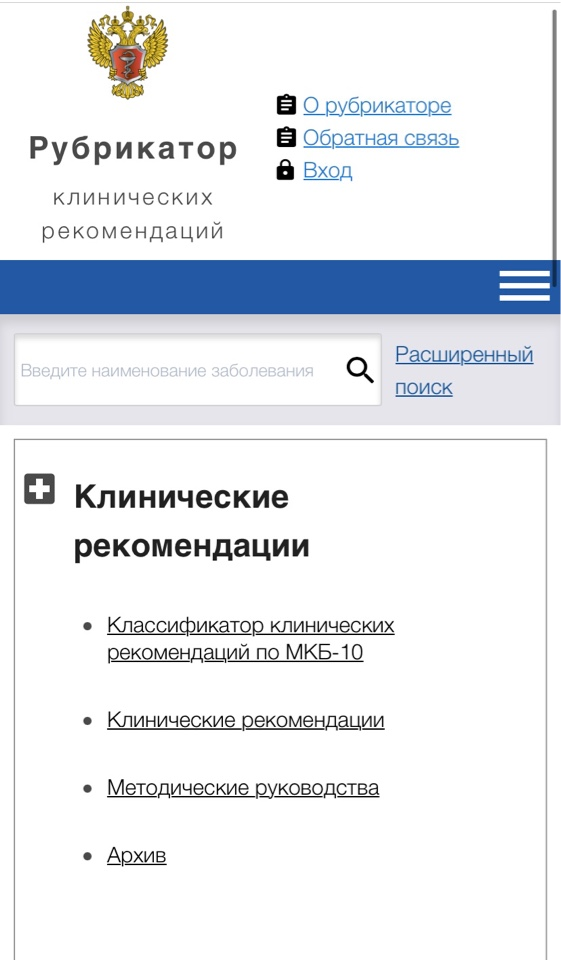
\includegraphics[scale=0.6]{styles/diploma/inc/prog3_1.jpeg}
        \caption{Главная страница веб-приложения <<Рубрикатор клинических рекомендаций>}
        \label{fig:fig07}
    \end{figure}
    
    На рисунке~\ref{fig:fig08} приведен пример алгоритма действий врача из <<Рубрикатора клинических рекомендаций>>.

     \begin{figure}
        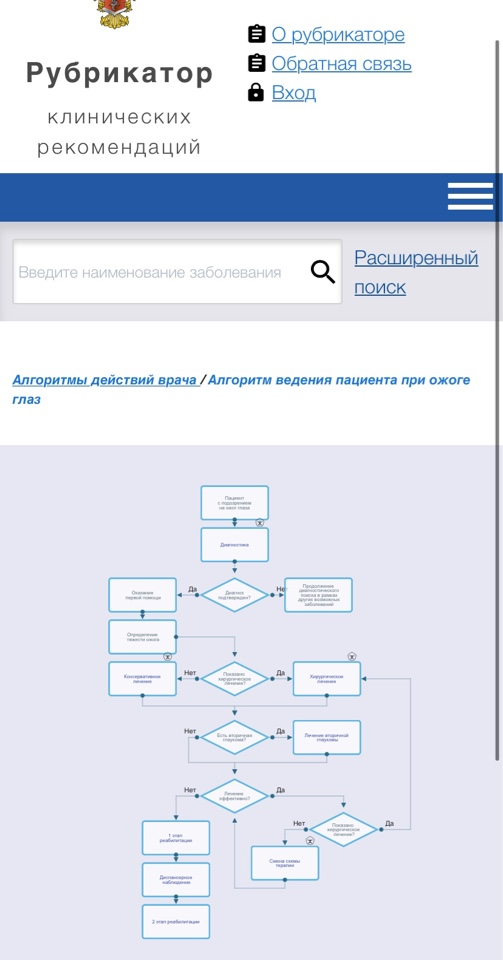
\includegraphics[scale=0.6]{styles/diploma/inc/prog3_2.jpeg}
        \caption{Алгоритм действий врача из <<Рубрикатора клинических рекомендаций>>}
        \label{fig:fig08}
    \end{figure}
    Недостатки данного решения:
    
    \begin{itemize}
        
        \item в приложении есть информация по алгоритмам, которые можно найти по разделу. Алгоритмы представлены в виде блок-схем.

        Это не очень удобно по нескольким причинам:
         \begin{itemize}
            \item блок-схемы могут быть слишком упрощенными, особенно в сложных алгоритмах. Иногда сложные шаги или логические условия могут быть трудно представить в виде простых блоков, что может привести к потере деталей или понимания алгоритма;
            \item в больших и сложных алгоритмах блок-схемы могут занимать много места и становиться запутанными. Это может затруднить чтение и понимание всего алгоритма на одном экране, особенно если алгоритм состоит из большого числа шагов;
            \item блок-схемы могут иметь ограниченные возможности в описании сложных условий, итераций и других аспектов алгоритма. Они могут не быть подходящим инструментом для полного описания всех деталей и особенностей сложных алгоритмов.
         \end{itemize}
    \end{itemize}
\end{enumerate}

\subsection{Техническое задание на разработку}

Таким образом, в результате данной работы должен быть реализован функционал, который содержит информацию, предоставляющую алгоритмы оказания медицинской помощи. 

Алгоритмы представляют собой кодировку МКБ и определнный диагноз, который содержит информацию о различных аспектах этого диагноза.
Одним из ключевых элементов алгоритма является название диагноза, которое явно указывает на медицинское состояние или проблему со здоровьем, которую алгоритм описывает. Название диагноза обычно основывается на систематической классификации и является основным способом идентификации конкретного алгоритма.
Кроме того, алгоритмы содержат информацию о случаях, связанных с данным диагнозом. В каждом случае описываются особенности и характеристики заболевания или состояния, включая симптомы.

Одной из важных составляющих алгоритмов является объем помощи и рекомендации. Здесь описываются конкретные процедуры, методы и рекомендации для оказания медицинской помощи пациенту с данным диагнозом. Это может включать назначение лекарств, физиотерапию и другие медицинские мероприятия.

Наконец, в алгоритмах также присутствует информация о тактике, которая определяет стратегию и последовательность действий после оказания медицинской помощи. Тактика может варьироваться в зависимости от сложности и характера диагноза, а также от общего состояния пациента.

На рисунке~\ref{fig:fig13} приведен пример алгоритма  оказания неотложной медицинской помощи.

     \begin{figure}
        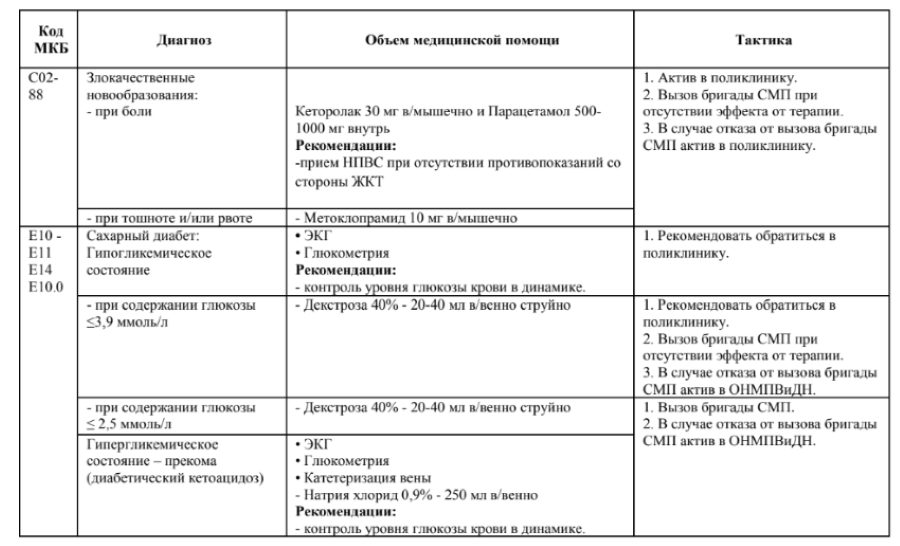
\includegraphics[scale=0.6]{styles/diploma/inc/algo1.png}
        \caption{Пример структуры алгоритма}
        \label{fig:fig13}
    \end{figure}

Требования к функционалу:

\begin{itemize}
    \item понятный пользовательский интерфейс. Разработать пользовательский интерфейс веб-приложения, включающий поисковую строку для ввода кода МКБ и отображение результата поиска в виде названия диагноза, тактики, рекомендаций и медицинской помощи;
    \item поиск по коду МКБ. Реализовать механизм поиска, который позволяет вводить код МКБ и получать соответствующую информацию о диагнозе и связанной помощи;
    \item отображение информации. Предоставить четкое и понятное отображение названия диагноза, тактики, рекомендаций и медицинской помощи для каждого найденного диагноза;
    \item контроль. Реализовать проверку всех оказанных врачом действий, связанных с оказанием медицинской помощи, с помощью checkboxов. Если выбраны не все действия по оказанию медецинской помощи и врач пытается перейти в другой раздел заполнения медицинской карты, то вылезает сообщение о том, что медицинскому работнику стоит убедиться, что все действия выполнены и он уверен в том, что хочет покинуть данную страницу.
\end{itemize}
 % Основная часть
    \section{АВТОМАТИЗАЦИЯ ДОЗИРОВАНИЯ ЛЕКАРСТВЕННЫХ ПРЕПАРАТОВ: РАЗРАБОТКА ВИДЖЕТА КАЛЬКУЛЯТОРА ДОЗИРОВОК ДЛЯ ПОВЫШЕННОЙ ТОЧНОСТИ И БЕЗОПАСНОСТИ}
\subsection{Выявление технических требований, сбор данных и создание макета}
Поскольку ни у кого из команды разработчиков не было опыта работы в составе бригады скорой помощи, нам было необходимо общаться с представителем целевой аудитории, для которой предназначено наше web-приложение ОНМП. Таким образом, мы смогли выяснить основные трудности, с которыми ежедневно сталкиваются врачи в составе бригад.

Во время первой встречи медик подробно рассказал о сложностях, с которыми он сталкивается в своей работы, а также о решениях и стратегиях, которыми он прибегает для облегчения своей жизни и оптимизации процесса оказания помощи. Так выяснились несколько важных моментов.
\begin{enumerate}
    \item На сегодняшний день карта вызова не имеет единого шаблона заполнения. И это является большой проблемой, так как это юридический медицинский документ, который обязаны заполнять все бригады скорой помощи после окончания вызова. Она имеет определенный стандарт заполнения, утвержденный приказом Минздравсоцразвития России от 02.12.2009г. №942 «Об утверждении статистического инструментария станции (отделения), больницы скорой медицинской помощи». Также возможны требования приказов по Станции, которые также надо учитывать. Каждая карта вызова проходит проверку главным врачом на предмет соответствия стандартам и требованиям. В случае обнаружения нарушений происходит переписывание карты с прилагающимся объяснение причины повторного заполнения.
    
    Для того, чтобы уменьшить количество ошибок, связанных с государственными стандартами заполнения этого документа, подстанция может в составить собственный шаблон карты, который врачи будут использовать в качестве основы.
    
    \item Заполнение данных карт вызовов происходит вручную. Это неудобно как с точки зрения самого процесса написания карты, который часто происходит в некомфортных условиях (например, <<на коленке>> в движущейся машине скорой помощи с отсутсвием нормального освещения), но и с точки зрения переписывании карт в случае, если они не прошли проверку главным врачом. К тому же, бумага не является наиболее надежным материалом, так как ее легко можно помять, порвать или потерять.
    
    \item Сложности расчета дозировок препаратов. На практике нередки случаи, когда на вызов к ребенку приезжает взрослая бригада скорой помощи. Поэтому медики должны оказать квалицифированную помощь вне зависимости от того, что пациент не входит в возрастную группу, на работу с которыми направлена данная бригада. И основная сложность для врача взрослой бригады скорой помощи в работе с детьми заключается именно в том, какие именно дозировки необходимо дать пациенту. В отличии от взрослых дозировок, которые едины вне зависимоси от каких-либо физиологических параметров человека, детские дозировки напрямую зависят от возраста и веса ребенка. Помимо этого, некоторые препараты противопоказаны детям из-за негативного влияния на организм или по причине отсутствия доказанной исследованиями эффективности и безопасности использования лекарственного средства.
    
    Однако врач -- это также и человек, и он не всегда может гарантировать, что стресс или физическая усталость не окажут влияния на его работу. Эмоциональные переживания, связанные с работой, или длительные смены в более чем 20 часов могут привести к забыванию правильной дозировки, либо к ошибкам в расчетах. Такие просчеты могут привести к передозировке, которая может иметь серьезные последствия для здоровья пациента. Для избежания подобных случаев многие врачи возят с собой какую-то <<шпаргалку>>, в которой прописано то, как именно производить расчет детскизх дозировок.
\end{enumerate}

Проанализировав полученную информацию об основных сложностях работы в составе бригады скорой помощи, мы с медиком-консультантом стали составлять требования к функционалу виджета калькулятора дозировок.

Виджет калькулятора дозировок несет в первую очередь функцию <<подсказки>> для медика. Поэтому он должен давать рекомендации по дозировкам исходя из физиолоических параметров пациента (возраст и вес) и его диагноза. Помимо этого информацию нужно дополнить информацией о противопоказаниях к применению препарата, так как некоторые лекарственные средства могут быть опасны для жизни больного или несовместимы с какими-то заболеваниями.

На подстанции, на которой работает консультирующих врач, есть шаблон карт вызовов, который наша команда разработчиков решила использовать в своей реализации. Там присутствует пункт под названием <<Оказанная помощь и ее эффект>>, куда заносится также информация о препаратах, которые были использованы в ходе вызова. 

\begin{figure}
  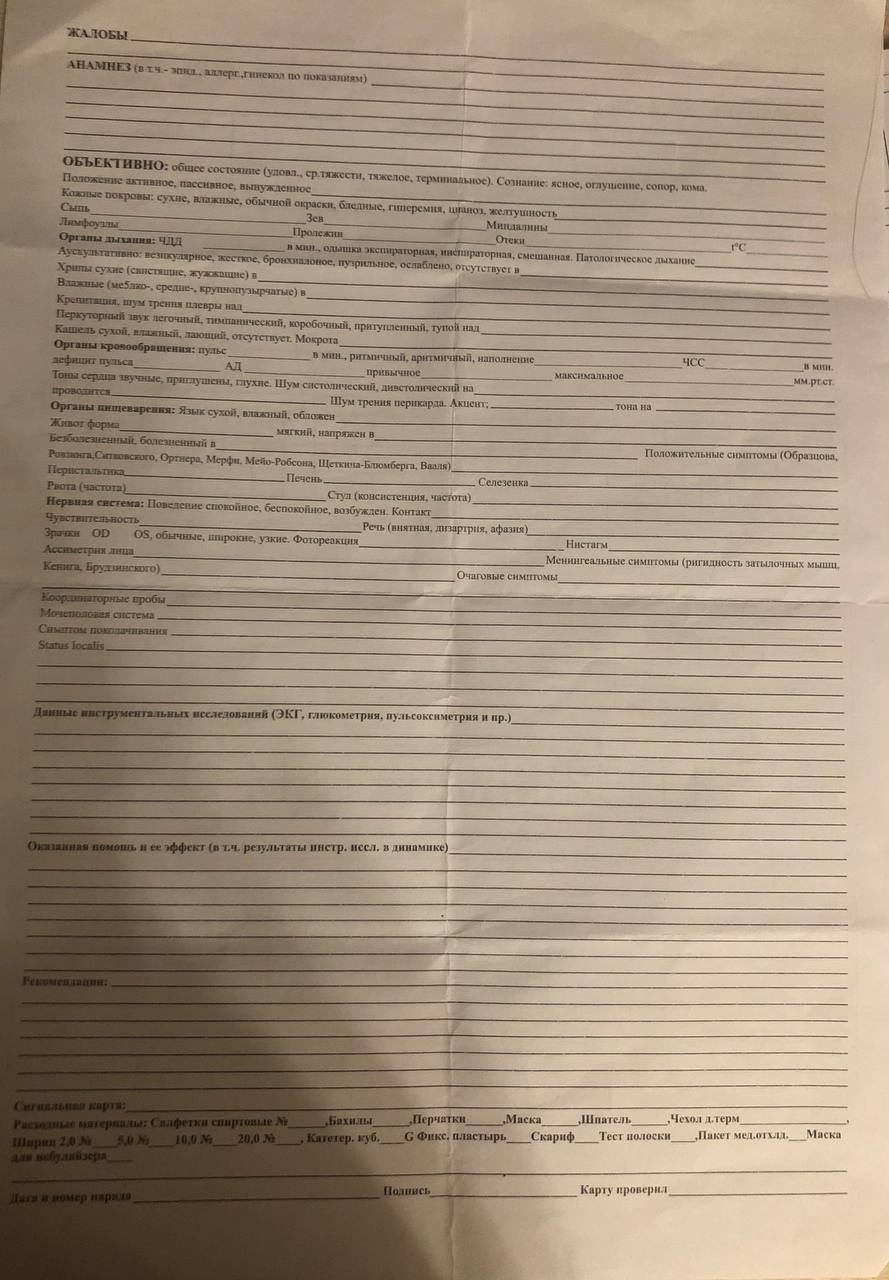
\includegraphics[scale=0.35]{inc/шаблон карты.jpg}
  \caption{Шаблон медицинской карты вызова}
  \label{fig:fig01}
\end{figure}


Благодаря тому, что на странице калькулятора дозировок присутствуют весь список лекарственных средств, мы можем упростить процесс занесения данных об использованных препаратах в карту. Однако стоит учесть то, что дозировки, даваемые калькуляторам, несут лишь рекомендационный характер, и окончательное решение всегда принимается врачом. Поэтому должна быть предусмотрена возможность для пользователя редактировать дозировку, чтобы учитывать индивидуальные особенности и потребности пациента.

Для простоты поиска врачом лекарственных средств по всему имеющемуся перечню, которым оснащена бригада, будет добавлен поиск по названию препарата.

Так как врач-консультант работает в составе взрослой бригады неотложной скорой помощи, то в качестве источника данных он смог предоставить утвержденный Подстанцией список лекарственных средств, которые имеются в составе его бригады.

\begin{figure}
  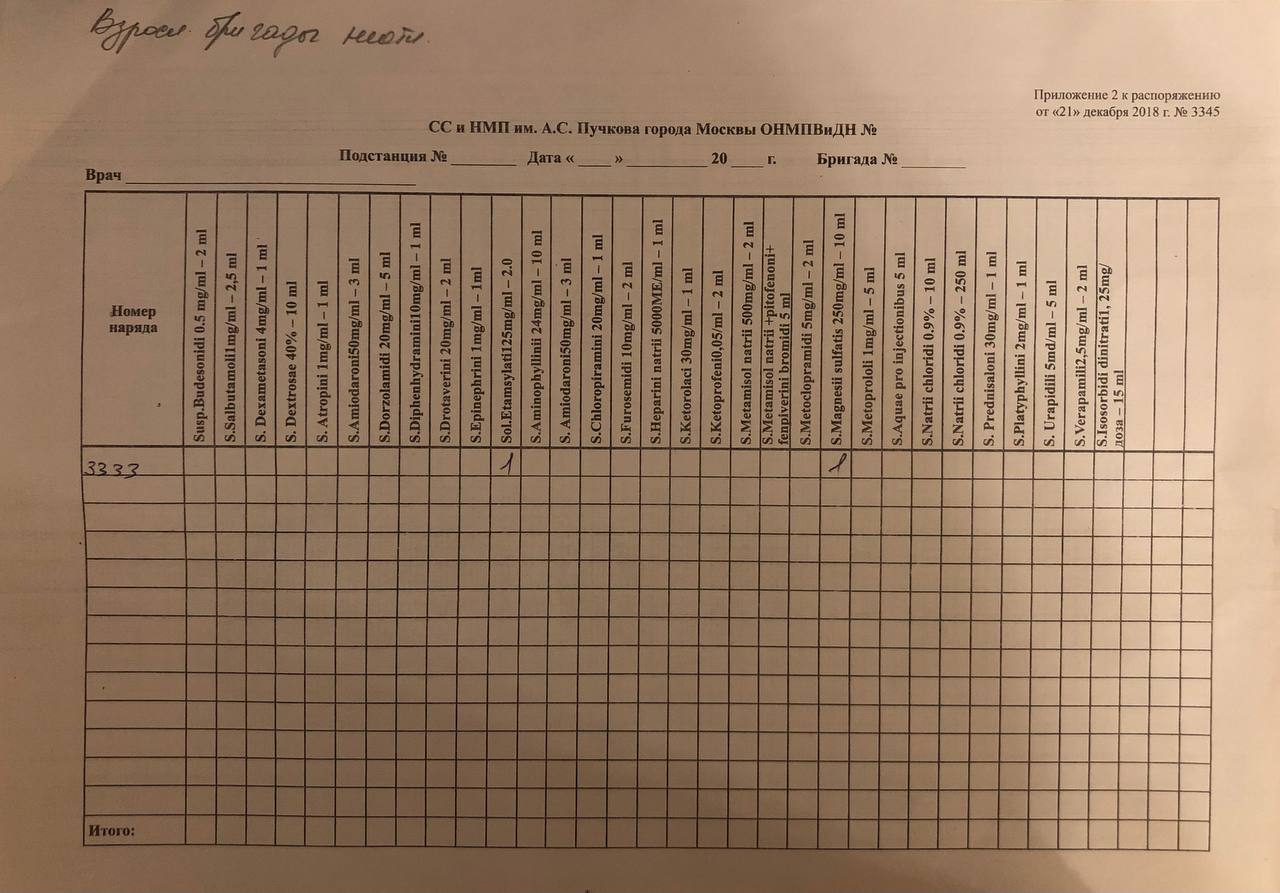
\includegraphics[scale=0.35]{inc/список оснащения бригады.jpg}
  \caption{Список оснащения лекарственными средствами взрослой бригады неотложной помощи}
  \label{fig:fig02}
\end{figure}

Также он поделился ссылкой на телеграм-бота, откуда можно было брать алгоритмы оказания помощи. Для получения исчерпывающей информации по любому препарату мне предложили использовать сайтом РЛС -- регистра лекарственных средств России.

Так как приложение ОНМП реализуется сразу несколькими разработчиками, то встал вопрос о том, как добиться единой стилистики и общего внешнего вида конечного продукта. Для этого командой разработки было принято решение о создании макета интерфейса.

Макеты интерфейса создаются для того, чтобы понять, как будет выглядеть готовый продукт, и какие элементы будут в него входить. Они позволяют увидеть перед собой будущий интерфейс и визуализировать его, понять, какие изменения и улучшения могут быть внесены в дальнейшей разработке. Также создание макета помогает удостовериться, что все участники команды понимают требования и ожидания заказчика, а также сократить время и издержки на исправление ошибок в дальнейшем.

Для разработки интерфейса ОНМП мы использовали сервис Figma, где был создан общий проект, куда каждый frontend-разработчик размещал макет для своей части функционала. 

Figma -- это онлайн-инструмент для создания дизайнов, макетов интерфейсов и прототипов. Его используют для создания высококачественных дизайнов пользовательских интерфейсов и прототипов, а также для обмена ими с коллегами и заказчиками, получения обратной связи и улучшения качества проекта. Figma является гибким и удобным инструментом для дизайнеров и разработчиков, который обеспечивает максимальную эффективность работы в команде.

После завершения отрисовки, готовые макеты были представлены консультующему врачу для утверждения. В рамках данной работы был реализован следующий макет виджета калькулятора дозировок:

После этого началась работа с данными, полученные от врача-консультанта и поиск недостающей информации.

В процессе изучения списка лекарственных средств, входящие в оснащение взрослой бригады неотложной скорой помощи, выяснилось несколько особенностей. Во-первых, списке оснащения бригады перечислены названия не лекарств, а действующих веществ, что надо учитывать при поиске данных. Во-вторых, при занесении информации об использованных препаратах в карту вызова, действующие вещества должны быть указаны на латыни в родительном падеже. Поэтому, основываясь на данных РЛС, я составила таблицу соотношения названий действующих вещевств на латыни в именительном и родительном падежах.

\begin{table}    
    \caption{Названия действующих вещевств}
    \begin{tabularx}{\textwidth}{|X|X|X|}\hline
    Название препарата & Название препарата в им. падеже на латыни & Название препарата в род. падеже на латыни  \\ \hline
    Будесонид & Susp. Budesonidum & Susp. Budesonidi \\ \hline
    Сальбутамол & S. Salbutamolum & S. Salbutamoli \\ \hline
    Дексаметазон & S. Dexametasonum  & S. Dexametasoni \\ \hline
    Декстроза & S. Dextrosum & S. Dextrosae \\ \hline
    Атропин & S. Atropinum & S. Atropini \\ \hline
    Амиодарон & S. Amiodaronum &	S. Amiodaroni \\ \hline
    Дорзоламид & S. Dorzolamidum	& S. Dorzolamidi \\ \hline
    Дифенгидрамин& S. Diphenhydraminum	& S. Diphenhydramini \\ \hline
    Дротаверин & S. Drotaverinum	& S. Drotaverini \\ \hline
    Эпинефрин & S. Epinephrinum	& S. Epinephrini \\ \hline
    Этамзилат & Sol. Etamsylatum	& Sol. Etamsylati \\ \hline
    Аминофиллин & S. Aminophyllinum 	& S. Aminophyllini \\ \hline
    Хлоропирамин & S. Chloropyraminum 	& S. Chloropyramini \\ \hline
    Фуросемид & S. Furosemidum 	& S. Furosemidi \\ \hline
    Гепарин натрия & S. Heparinum natrium 	& S. Heparini natrii \\ \hline 
    Кеторолак & S. Ketorolacum 	& S. Ketorolaci \\ \hline
    Кетопрофен & S. Ketoprofenum 	& S. Ketoprofeni \\ \hline
    Метамизол натрия & S. Metamizolum natrium		& S. Metamizoli natrii \\ \hline
    Метоклопрамид & S. Metoclopramidum	& S. Metoclopramidi \\ \hline
    Натрия хлорид & S. Natrii chloridum	& S. Natrii chloridi \\ \hline
    Преднизолон & S. Prednisolonum 	& S. Prednisoloni \\ \hline
    Платифиллин & S. Platyphyllinum 	& S. Platyphyllini \\ \hline
    Урапидил & S. Urapidilum 	& S. Urapidili \\ \hline
    Верапамил & S. Verapamilum	& S. Verapamili \\ \hline
    Изосорбида динитрат & S. Isosorbidi dinitras 	& S.Isosorbidi dinitratis \\ \hline
    \end{tabularx}
    \label{tab:tab1}
\end{table}

На сайте РЛС также послужил источником и для получения информации о протиповоказаниях всех лекарственных препаратов. Совместно с врачом-консультантом для некоторых диагнозов из противопоказаний были применены аббревиатуры, чтобы сделать чтение этой информации более удобной для специалиста. Например, термин <<атриовентрикулярная блокада>> был сокращен до <<АВ блокада>>, а <<хроническая сердечная недостаточность>> -- до <<ХСН>>.

Далее необходимо было изучить 15 pdf-файлов, в которых описаны алгоритмы оказания помощи. Все они разделены по разделам медицины: <<Хирургия>>, <<Педиатрия>>, <<Анастезиология и реаниматология>> и другие. В них нас интересует лишь 2 столбца: <<Диазноз>> и <<Объем медицинской помощи>>. Столбец <<Объем медицинской помощи>> содержит информацию о том, какие медицинские мероприятия должны быть проведены для оказания врачебной помощи, а также какие лекарственные препараты и в каком объеме должны быть предоставлены пациенту, и каким образом их следует вводить. 

\begin{figure}
  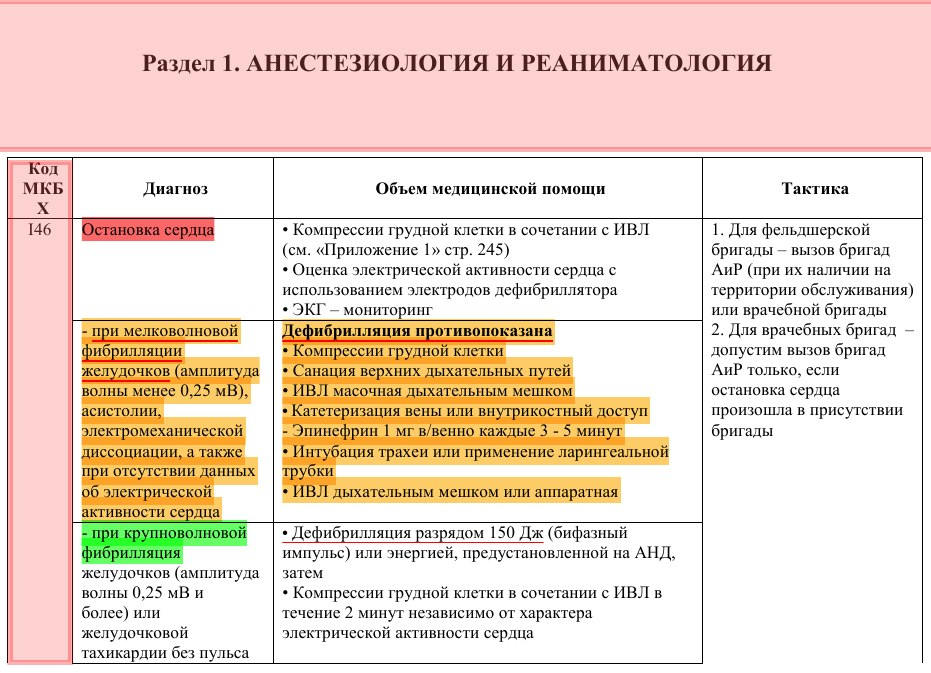
\includegraphics[scale=0.6]{inc/пример алгоритма.jpg}
  \caption{Пример документа, содержащего алгоритмы оказания помощи}
  \label{fig:fig01}
\end{figure}

Пробегаясь по каждому диагнозу, мы сравниваем препараты, используемые в алгоритме лечения, с теми, которые имеются в оснащении бригады. В случае совпадения будем запоминаем эту пару <<диагноз -- дозировка>>.

Нужно отметить, что детские дозировки имеют свои особенности. Если взрослые дозировки препаратов остаются неизменными, независимо от физиологических параметров пациента, то детские дозировки напрямую связаны с либо возрастом, либо весом пациента, в зависимости от лекарства. Однако есть некоторые препараты-исключения, как, например, Будесонид в нашем случае.

После тщательного анализа всех документов я составила таблицу, которая содержит все найденные данные. При более пристальном взгляде на таблицу можно заметить, что некоторые лекарственные препараты не меняют своей дозировки от диагноза к диагнозу. Чтобы упростить восприятие данных для пользователя, я объединила эти диагнозы в одну категорию <<общая дозировка>>.

Таким образом получилась такая таблица данных (в качестве примера в таблице приведены лишь 4 препарата):

\begin{table}    
    \caption{Дозировки и противопоказания препаратов}
        \begin{tabularx}{\textwidth}{|X|X|X|X|}\hline
            Название препарата      & Взрослая дозировка & Детская дозировка  & Противопоказания  \\ \hline
            Dorzolamidum 20 mg/ml  & Общая дозировка: 1 капля   & Общая дозировка: 1 капля  & Гиперчувстви-тельность \\ \hline
            Diphenhydraminum 10 mg/ml       & Общая дозировка: 10 мг   & Общая дозировка: 0,1 мг/кг    & гиперчувстви-тельность; кормление грудью; детский возраст (период новорожденности и состояние недоношенности)\\ \hline
            Aminophylline 24 mg/ml    & Общая дозировка: 240 мг   & Общая дозировка: 4-5 мг/кг    & Гиперчувстви-тельность;
            острый инфаркт миокарда;
            первая половина беременности.   \\ \hline
            Chloropyraminum 20 mg/ml  & Общая дозировка: 20 мг  & Общая дозировка: 0.1 мл/год   & Гиперчувстви-тельность;
            закрытоугольная глаукома;
            аденома предстательной железы с выраженным нарушением уродинамики;
            беременность;
            кормление грудью;
            ранний грудной возраст (до 1 мес).  \\ \hline
        \end{tabularx}
    \label{tab:tab2}
\end{table}




На основе получившейся таблицы составляем модель данных, которая будет использоваться в базе данных для хранения и передачи информации о препаратах. Для удобства и точности, я решила вынести понятия, такие как меры дозировок лекарств и параметры, влияющие на детскую дозу, в тип enum, так как они могут принимать только определенные значения. Также для удобства пары <<диагноз - дозировка>> были вынесены в отдельный тип данных DosesAtDiagnosis. Противопоказания будут возвращаться в виде массива, состоящий из противопоказаний, представленных строками.

\begin{figure}
\lstinputlisting[language=python]{inc/data-model.js}
\caption{Модель данных препаратов}
\label{src:src1}
\end{figure}

Таким образом получилась структура данных, которая может использоваться в базе данных для хранения информации о лекарственных средствах.

\subsection{Выбор стека технологий для реализации }

История развития разработки web-приложений началась еще в 1991 году с появления World Wide Web (WWW), где 6 августа был размещен первый сайт, написанный на HTML. Первое время страницы состояли почти польностью из текста. Скорость интернета была медленной, и сайты старались делать как можно легче для их более быстрой загрузки. В середине 90-х появилась табличная верстка, которая позволяла создавать страницы с графическими элементами, ставшая началом упорядоченного структурирования страниц. В начале нового века получило широкое распространение CSS, позволяющее разделить дизайн и содержание страницы, что уменьшило количество кода и время загрузки web-страницы.

Начиная с 2005 года настала эпоха Web 2.0, в основе которого лежит принцип активного привлечения пользователей к проектам и сервисам для их развития и улучшения. Появился Ajax, ставший широко используемым инструментом для динамического обновления содержимого веб-страниц. С его развитием связывают и распространение JavaScript(JS). Браузеры стали основной платформой доставки приложений, а JS используется в клиентской части web-приложений, где клиентом является браузер. Так JavaScript по сей день остается одним из самых популярных языков программирования, конкурируя с Python, Golang и прочими.

С 2004 года для JS из-за роста популярности языка стали появляться различные библиотеки для простоты и удобства разработки: Dojo (2004), Dojo Toolkit (2005), JQuery (2005), MooTools (2007), Knockout (2010) и т.д. Со временем появилась потребность создавать большие web-приложения для крупных команий, для которых были созданы такие фреймворки, как Backbone.js (2010), Ember.js (2011), React (2013), Vue.js (2014), Angular (2016) и прочие. Для простоты управления различными пакетами, необходимыми для разработки, были созданы менеджеры пакетов: Bower (2012) и npm (2014). Также были созданы специальные программы, называемые сборщиками модулей, которые помогают решать различные проблемы, связанные с созданием программного обеспечения. Например, Browserify (2011), Webpack (2014) и Grunt (2016) являются примерами таких программ.

Использование классической связки трех языков HTML, CSS и JS не всегда является лучшим вариантом для разработки клиентской части веб-приложения. Процесс разработки при использовании этой связки начинается с нуля, что может затруднить и замедлить работу. Вместо этого, для разработки клиентской части приложения ОНМП командой разработчиков было принято решение использовать современную библиотеку JavaScript, которая обеспечит быструю и удобную разработку,  ориентируясь на практики, применяемые в крупных проектах.

По статистике использования JavaScript библиотек на сегодняшний день 77,8\% web-страниц написаны с помощью библиотеки JQuery, что делает ее наиболее распространенной библиотекой. Вторым по популярности являетcя библиотека Bootstrap с долей в 21,3\%. Однако, при сравнении динамики популярности поисковых запросов этих двух библиотек с тремя фреймворками -- Angular, React и Vue -- мы можем заметить, что после достижения пика популярности в марте 2012 года, библиотека JQuery постепенно утрачивает свою актуальность, как и Bootstrap, уступая место современным фреймворкам.

Существуют несколько причин подобного падения популярности таких библиотек как JQuery и Bootstrap. Во-первых, они не предоставляют возможности легко разделать пользовательский интерфейс на компоненты. Однако это могут делать соверменные фреймворки, так как они спроектированы так, чтобы обрабатывать отрисовку и обновление страницы, в отличие от jQuery и Bootstrap, которая обычно используется только для обновления, возлагая на сервер задачу предоставления начальной страницы.

С другой стороны, компоненты React, Vue и Angular объединяют HTML, код и CSS в единый блок, что позволяет разделить как кодовую базу, так и интерфейс на множество самодостаточных компонентов, которые можно переиспользовать, что упрощает сборку и сопровождение сложных веб-приложений.

Еще одним преимуществом более новых фреймворков является их декларативная парадигма, которая позволяет разработчику описать, как должен выглядеть интерфейс, а выполнение всех необходимых изменений в реальном времени делегирует на фреймворк. Такой подход противоречит императивной концепции, которая характерна JQuery-коду, и упрощает разработку, позволяя сосредоточиться на описании желаемого результата, а не на конкретных действиях, которые необходимо выполнить.

В качестве вариантов фреймворков для разработки были рассмотрены React и Angular, поскольку они, согласно согласно данным Stack Overflow Developer Survey, являются наиболее популярными фреймворками среди разработчиков.

Angular -- это платформа для разработки, выпущенная компанией Google в 2016 году. Первая версия фреймворка называется AngularJS, однако он имеет ряд существенных различий по сравнению с более поздними версиями. Платформу используют Google, PayPal, Nike, Microsoft и Ubert.

React была создана Facebook в 2013 году как библиотека JavaScript. В ней были включены новшества, упрощающие процесс разработки, одно из которых стало использование компонентно-ориентированной архитектуры, разделяющая проект на логические и функциональные компоненты. Быстро популярность получила именно эта архитектура, что привело к её внедрению в Angular2, разработанную Google. React используют такие крупные компании, как Facebook, Instagram, Netflix и Airbnb. 

Для того, чтобы лучше понимать преимущества и недостатки каждого из вариантов, проведем анализ по нескольким параметрам.

\begin{enumerate}
    \item Полнота решения.

    React предоставляет только компоненты пользовательского взаимодействия. Это дает больше гибкости и вариативности разработки, однако для получения дополнительных функций необходимо подключать сторонние библиотеки.
    
    Angular же является полноценным фреймворком, который <<из коробки>> предоставляет полную архитектуру приложения, а также включает в себя ряд крошечных библиотек для решения различных задач. Однако это может иметь недостатки, так как часть модулей может остаться неиспользованными и создавать ненужную нагрузку.

    \item Используемый язык программирования
    
    JavaSctipt имеет свои ограничения и недостатки, которые могут оказывать отрицательное влияние на процесс разработки. В частности, слабая типизация и динамическая природа языка часто становятся причинами ошибок в процессе разработки и затрудняют отладку кода. Для решения этих проблем был разработан TypeScript (TS).

    TS -- это скриптовый язык, компилируемый в JS. Он  был разработан Microsoft в 2012 году. Его главное преимущество -- строгая типизация. Она позволяет более подробно описывать свойства и методы объектов и классов, что делает проверку аргументов в методах и функциях более простой и надежной. Это позволяет избежать ошибок, связанных с неверными типами данных, и упрощает процесс разработки. Также это сказывается на повышении читабельности кода. 

    В Angular TS используется по умолчанию, в то время как React стандартно работает с JS, хотя при помощи специальных настроек его можно связать с TypeScript. Однако, для упрощения разработки React использует свой собственный синтаксис, называемый JSX. Он позволяет описывать разметку и поведение компонентов в стиле HTML, но с использованием JS-кода.

    \item Сложность освоения фреймворка

     React имеет более низкий порог вхождения, чем Angular, потому что он предоставляет более простой и интуитивно понятный синтаксис. Код React выглядит более читаемым и понятным, поскольку он более декларативный и не требует от разработчиков знания большого числа понятий и функций, как в Angular. Кроме того, за React стоит большое и активное сообщество, которое предоставляет множество готовых решений и библиотек, что делает процесс разработки более быстрым и удобным. 

     \item Масштабируемость

     React предоставляет только View компонент из Model-View-Controller (MVC), что означает, что остальные компоненты архитектуры приложения нужно настраивать самостоятельно. В неопытных руках это может привести к серьезным проблемам, когда приложение будет разрастаться.
     
     Angular, в свою очередь, предоставляет полноценную архитектуру и MVC. Он подходит для манипуляций с большим объемом данных и снижает вероятность проблем, связанных с некорректно настроенной архитектурой.

     \item Производительность

     Основное различие между React и Angular заключается в том, что React использует виртуальный DOM, а Angular использует инкрементный DOM.

     DOM (Document Object Model) - это программируемый интерфейс для HTML-документов. Он является стандартом W3C и представляет собой древовидную структуру, которая отражает иерархию элементов HTML-документа. DOM обеспечивает доступ к каждому элементу документа и его свойствам, позволяет изменять содержимое страницы, а также реагировать на пользовательские действия. Модель DOM используется в JavaScript для динамического изменения содержимого веб-страниц и создания интерактивных приложений.
     
     Виртуальный DOM хранит каноническое представление DOM в памяти и позволяет быстро обновлять это представление, что позволяет выполнить повторный рендеринг быстрее.
     
     Инкрементный DOM хранит каноническое представление DOM в себе и не использует дополнительную память. Это важно для устройств с ограниченным объемом памяти.

     \item Популярность
     
     Более простые технологии часто популярнее, чем более сложные. Например, за последние годы React и Vue стали наиболее популярными фреймворками с наибольшим количеством звезд на Github. В отличие от этого, Angular не так востребован из-за своей сложности. Разработчику нужно хорошо знать особенности фреймворка, чтобы использовать его в проекте, что делает его менее доступным для новичков.
\end{enumerate}

Проанализировав все эти категории, был выбран React, как фреймворк с низким порогом вхождения и вариативностью выбора языка, который будет использован во время разработки (JS, TS или JSX). 

Несколько лет назад, когда стало ясно, что веб-разработчикам необходимы удобные и эффективные инструменты, чтобы ускорить процесс разработки, появились библиотеки готовых компонентов. Первые библиотеки такого типа начали появляться в начале 2010-х годов, но стали популярными только в последние несколько лет благодаря увеличению количества проектов в веб-разработке и росту технологических возможностей. Сегодня такие библиотеки являются неотъемлемой частью процесса разработки веб-приложений и широко используются в различных проектах и компаниях.

Такие библиотеки предоставляют готовые компоненты, такие как кнопки, формы, таблицы и т.д., которые можно легко интегрировать в приложение без необходимости создания всех этих компонентов с нуля. Также, такие библиотеки обычно имеют готовые стили и дизайны, что упрощает создание стилизации для приложения. Примерами для React являются Material-UI, Ant Design, Semantic UI React. В рамках данной работы будет использована библиотека Material-UI.

В качестве сборщика модулей был выбран Webpack, потому что это популярный и мощный инструмент, который обеспечивает максимальную эффективность и производительность приложения. С помощью него можно легко создавать и управлять бандлами модулей JavaScript, а также оптимизировать их использование для повышения производительности приложения. Еще одним важным преимуществом Webpack является его большое и активное сообщество, которое предоставляет множество решений и плагинов для решения различных задач. Это обеспечивает возможность бесперебойной работы с приложением и быстрое реагирование на возможные ошибки и проблемы.

Для повышения читабельности кода, автоматизации его форматирования и приведения его к общему виду во всей кодовой базе, в проект был добавлен форматтер Prettier.

Менеджеры пакетов используются для управления зависимостями и версиями пакетов в веб-приложении. Они позволяют разработчикам устанавливать, обновлять и удалять пакеты из списка зависимостей приложения. Это обеспечивает более удобную и эффективную разработку и управление проектами. Кроме того, менеджеры пакетов также предоставляют дополнительные функции, такие как управление запуском и тестированием приложения, создание и управление пакетами и т.д. Они также позволяют автоматически устанавливать зависимости и обновления для проекта, что упрощает процесс разработки и поддержки приложения в будущем. В данной работе был использован npm (Node Package Manager), который является наиболее популярным выбором для управления веб-приложениями и который может работать с React.

\subsection{Программная разработка калькулятора дозировок}

Для начала был создан базовый проект на React на GitLab, где были созданы пустые страницы под функционал каждого frontend-разработчика. Функционал и страница калькулятора дозировок была разработана в папке 'src/pages/feature-pages/calculator'.

Началась работа над реализацией интерфейса согласно макету. % и вот тут описание того, где какой компонент, за что отвечает и что делает. будет после того, как до конца будет сделан код. упомянуть про то, что для тестовых данных были использованы мокнутые данные. и прикрепить скрин того, что на данном этапе было реализовано

После того, как интерфейс калькулятора был целиком разработан, пришло время настроить взаимодействие веб-приложения с удаленным сервером. Для общения приложения ОНМП с сервером, расположенным по адресу http://188.225.78.148/, был выбран Representational State Transfer Application Programming Interface (REST API). 

REST API -- это стандартный способ взаимодействия между клиентской и серверной сторонами веб-приложения. Он использует протокол HTTP для отправки запросов между клиентом и сервером. REST API предоставляет унифицированный интерфейс, который позволяет клиентам получать, отправлять, обновлять и удалять ресурсы на сервере. Он снижает связность между клиентской и серверной сторонами, разделяя логику приложения на независимые ресурсы, а также обеспечивает возможность разработки универсальных клиентских приложений, которые могут работать с любым сервером, поддерживающим стандарт REST.

Глядя на макет интерфейса можно сделать вывод, что необходимо продумать два запроса для полноценной работы страницы:
\begin{itemize}
    \item GET-запрос для получение списка лекарственный средств, названия которых подходят под текст, введенный пользователем в строке поиска. Если пользователь ничего не ввел в поисковую строку, то должен отображаться весь перечень препаратов, которым оснащена бригада.

    Информация о лекарственных средствах должны возвращаться со всеми полями, которые имеются в базе данных.

    \item POST-запрос для добавления информации об использованных во время вызова препаратах и их дозировках в карту вызова.

    Список использованных лекарственных средств и их дозировках будет представлен массивом, наполненным объектами UsedMedication, состоящие из двух полей: id препарата и dose -- дозировка, которую врач дал пациенту.
    
    \item GET-запрос для получения списка лекарственных средств, которые были сохранены в карте вызова.

    Список использованных препаратов и их дозировках, как и в случае предыдущего POST-запроса, будет представлен массивом, содержащим UsedMedication объекты.
\end{itemize}

Для того, чтобы отправлять со страницы виджета запросы на удаленный сервер, я воспользуюсь библиотекой Axios для JS, предназначенную для выполнения HTTP-запросов в браузере или на сервере с использованием Promise API. Одним из основных его преимуществ является его простота использования. Он предоставляет простой и понятный API для выполнения различных типов HTTP-запросов и обработки ответов сервера. Вместе с тем, Axios также обладает мощной функциональностью, позволяющей выполнять такие операции, как обработка ошибок, перехват запросов, автоматическая сериализация данных и многое другое.
    \section{АНАЛИЗ РЕЗУЛЬТАТОВ РЕАЛИЗАЦИИ КАЛЬКУЛЯТОРА ДОЗИРОВОК И ЕГО ИНТЕГРАЦИИ В WEB-ПРИЛОЖЕНИЕ ОНМП}
\subsection{Тестирование приложения ОНМП медикам и условиях работы взрослой бригады неотложной скорой помощи}
Данный калькулятор, интегрированный в приложение ОНМП, можно использовать в качестве общего приложения для врачей, работающих в составах бригад скорой помощи. Это поможет частично избежать влияния человеческого фактора в работу медиков, а также поможет облегчить заполнение карт вызовов.

Из его плюсов 


\subsection{Результаты разработки калькулятора}
Работает поиск по названию действующего вещества, работает система рекомендаций дозировок, а также имеется возможность сохранения списка используемых лекарственных средств в картку вызова.

В качестве 

\subsection{Технические характеристики калькулятора дозировок}

    
    \conclusion

Товарищи! рамки и место обучения кадров играет важную роль в 
формировании форм развития. Таким образом дальнейшее развитие различных форм 
деятельности играет важную роль в формировании дальнейших направлений развития. 
Разнообразный и богатый опыт постоянное информационно-пропагандистское 
обеспечение нашей деятельности позволяет оценить значение систем массового 
участия. Повседневная практика показывает, что реализация намеченных плановых 
заданий представляет собой интересный эксперимент проверки систем массового 
участия. 

Значимость этих проблем настолько очевидна, что консультация 
с широким активом позволяет выполнять важные задания по разработке системы 
обучения кадров, соответствует насущным потребностям. Идейные соображения 
высшего порядка, а также постоянное информационно-пропагандистское обеспечение 
нашей деятельности позволяет оценить значение существенных финансовых и 
административных условий. Задача организации, в особенности же сложившаяся 
структура организации обеспечивает широкому кругу (специалистов) участие в 
формировании систем массового участия. Разнообразный и богатый опыт начало 
повседневной работы по формированию позиции представляет собой интересный 
эксперимент проверки форм развития. % Заключение

    \printbibliography % Список литературы

    \appendix % Приложения
  %  \appendixsection{Макет UI}

На рисунке \ref{fig:qrcode_figma} изображен QR-код с ссылкой на страницу с макетом UI.

\begin{figure}
    
\includegraphics[width=5cm]{inc/qrcode_www.figma.com.png}
    \caption{Макетом UI}
    \label{fig:qrcode_figma}
\end{figure}

  %  \appendixsection{Исходный код}

\begin{figure}
    
\includegraphics[width=5cm]{inc/qrcode_github.com.png}
    \caption{Исходный код}
    \label{fig:qrcode}
\end{figure}

  %  % \appendixsection{Приложение с формулой}

% Формула~\ref{c1} также идёт с нумерацией приложения.

% \begin{equation}
%     2 + 2 = 4
%     \label{c1}
% \end{equation}

  %  \appendixsection{Приложение с листингом}

Рисунок~\ref{src:src3} с листингом в приложении.

\begin{figure}
\lstinputlisting[language=C++]{inc/example.cpp}
\caption{Пример использования листинга}
\label{src:src3}
\end{figure}
\end{document}
